\documentclass[a4paper,12pt]{article}
\usepackage[top = 2.5cm, bottom = 2.5cm, left = 2.5cm, right = 2.5cm]{geometry}
\usepackage[T1]{fontenc}
\usepackage[utf8]{inputenc}
\usepackage{multirow} 
\usepackage{booktabs} 
\usepackage{graphicx}
\usepackage[spanish]{babel}
\usepackage{setspace}
\setlength{\parindent}{0in}
\usepackage{float}
\usepackage{fancyhdr}
\usepackage{amsmath}
\usepackage{amssymb}
\usepackage{amsthm}
\usepackage[numbers]{natbib}
\newcommand\Mycite[1]{%
	\citeauthor{#1}~[\citeyear{#1}]}
\usepackage{graphicx}
\usepackage{subcaption}
\usepackage{booktabs}
\usepackage{etoolbox}
\usepackage{minibox}
\usepackage{hyperref}
\usepackage{xcolor}
\usepackage[skins]{tcolorbox}
%---------------------------

\newtcolorbox{cajita}[1][]{
	 #1
}

\newenvironment{sol}
{\renewcommand\qedsymbol{$\square$}\begin{proof}[\textbf{Solución.}]}
	{\end{proof}}

\newenvironment{dem}
{\renewcommand\qedsymbol{$\blacksquare$}\begin{proof}[\textbf{Demostración.}]}
	{\end{proof}}

\newtheorem{problema}{Problema}
\newtheorem{definicion}{Definición}
\newtheorem{ejemplo}{Ejemplo}
\newtheorem{teorema}{Teorema}
\newtheorem{corolario}{Corolario}[teorema]
\newtheorem{lema}[teorema]{Lema}
\newtheorem{prop}{Proposición}
\newtheorem*{nota}{\textbf{NOTA}}
\renewcommand\qedsymbol{$\blacksquare$}
\usepackage{svg}
\usepackage{tikz}
\usepackage[framemethod=default]{mdframed}
\global\mdfdefinestyle{exampledefault}{%
linecolor=lightgray,linewidth=1pt,%
leftmargin=1cm,rightmargin=1cm,
}




\newenvironment{noter}[1]{%
\mdfsetup{%
frametitle={\tikz\node[fill=white,rectangle,inner sep=0pt,outer sep=0pt]{#1};},
frametitleaboveskip=-0.5\ht\strutbox,
frametitlealignment=\raggedright
}%
\begin{mdframed}[style=exampledefault]
}{\end{mdframed}}
\newcommand{\linea}{\noindent\rule{\textwidth}{3pt}}
\newcommand{\linita}{\noindent\rule{\textwidth}{1pt}}

\AtBeginEnvironment{align}{\setcounter{equation}{0}}
\pagestyle{fancy}

\fancyhf{}









%----------------------------------------------------------
\lhead{\footnotesize Álgebra Moderna}
\rhead{\footnotesize  Rudik Roberto Rompich}
\cfoot{\footnotesize \thepage}


%--------------------------

\begin{document}
 \thispagestyle{empty} 
    \begin{tabular}{p{15.5cm}}
    \begin{tabbing}
    \textbf{Universidad del Valle de Guatemala} \\
    Departamento de Matemática\\
    Licenciatura en Matemática Aplicada\\\\
   \textbf{Estudiante:} Rudik Roberto Rompich\\
   \textbf{Correo:}  \href{mailto:rom19857@uvg.edu.gt}{rom19857@uvg.edu.gt}\\
   \textbf{Carné:} 19857
    \end{tabbing}
    \begin{center}
        MM2035 - Álgebra Moderna - Catedrático: Ricardo Barrientos\\
        \today
    \end{center}\\
    \hline
    \\
    \end{tabular} 
    \vspace*{0.3cm} 
    \begin{center} 
    {\Large \bf  Tarea 13
} 
        \vspace{2mm}
    \end{center}
    \vspace{0.4cm}
%--------------------------
\section{Tabla de valores para cada voltaje}

\begin{table}[H]
    \centering
    \begin{tabular}{@{}cccc@{}}
    \toprule
    \textbf{Voltaje} &  \textbf{ADC} &  \textbf{D (cm)} & \textbf{1/R (cm)} \\ \midrule
    100           & 0.851     & 8                     & 0.25                    \\
    100           & 1.561     & 5                     & 0.4                     \\
    100           & 2.012     & 3.5                   & 0.57142857              \\
    100           & 2.129     & 3.5                   & 0.57142857              \\
    100           & 1.479     & 5                     & 0.4                     \\
    120           & 1.054     & 7                     & 0.28571429              \\
    120           & 1.719     & 4.5                   & 0.44444444              \\
    120           & 2.392     & 3.5                   & 0.57142857              \\
    120           & 1.1798    & 4.5                   & 0.44444444              \\
    120           & 1.196     & 6.5                   & 0.30769231              \\
    140           & 0.768     & 10                    & 0.2                     \\
    140           & 0.99      & 7                     & 0.28571429              \\
    140           & 1.333     & 6                     & 0.33333333              \\
    140           & 1.801     & 4.5                   & 0.44444444              \\
    140           & 2.439     & 3.5                   & 0.57142857              \\
    160           & 0.887     & 10                    & 0.2                     \\
    160           & 1.146     & 7.5                   & 0.26666667              \\
    160           & 1.833     & 5                     & 0.4                     \\
    160           & 1.989     & 4.5                   & 0.44444444              \\
    160           & 1.433     & 6.5                   & 0.30769231              \\
    180           & 0.845     & 10.5                  & 0.19047619              \\
    180           & 1.349     & 7                     & 0.28571429              \\
    180           & 2.039     & 4.5                   & 0.44444444              \\
    180           & 1.742     & 6.5                   & 0.30769231              \\
    180           & 1.22      & 7.5                   & 0.26666667              \\
    200           & 0.833     & 11.5                  & 0.17391304              \\
    200           & 1.59      & 6                     & 0.33333333              \\
    200           & 2.41      & 4                     & 0.5                     \\
    200           & 1.822     & 5.5                   & 0.36363636              \\
    200           & 1.01      & 9.5                   & 0.21052632              \\ \bottomrule
    \end{tabular}
    \end{table}

    \section{Gráfico inverso del radio contra corriente para cada voltaje}
    \begin{figure}[H]
        \centering
        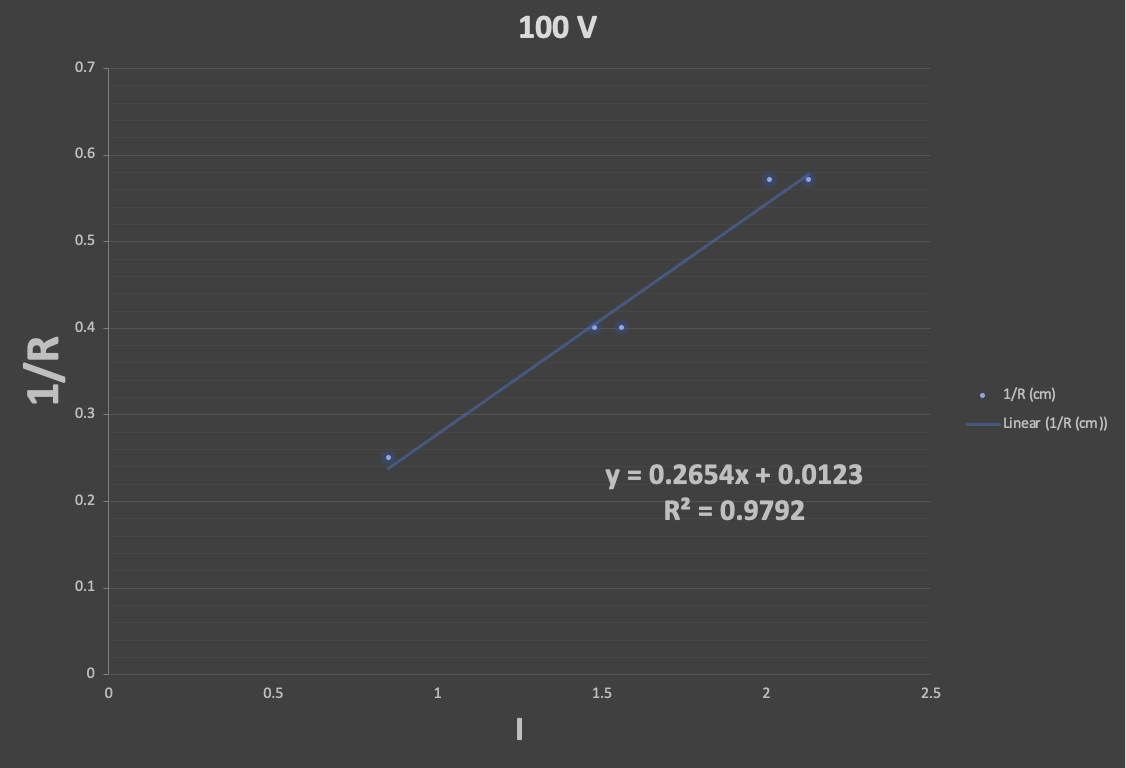
\includegraphics[scale=.7]{imagenes/1.png}
        \caption{100 V}
    \end{figure}
    \begin{figure}[H]
        \centering
        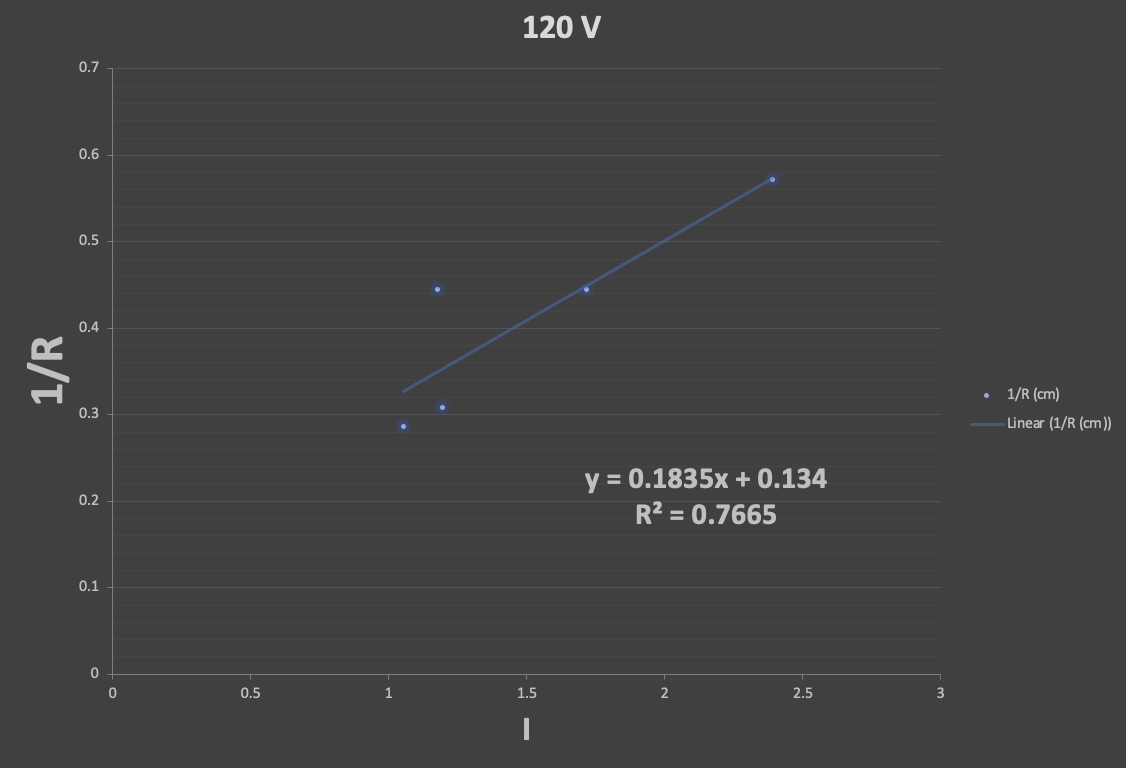
\includegraphics[scale=.7]{imagenes/2.png}
        \caption{120 V}
    \end{figure}
    \begin{figure}[H]
        \centering
        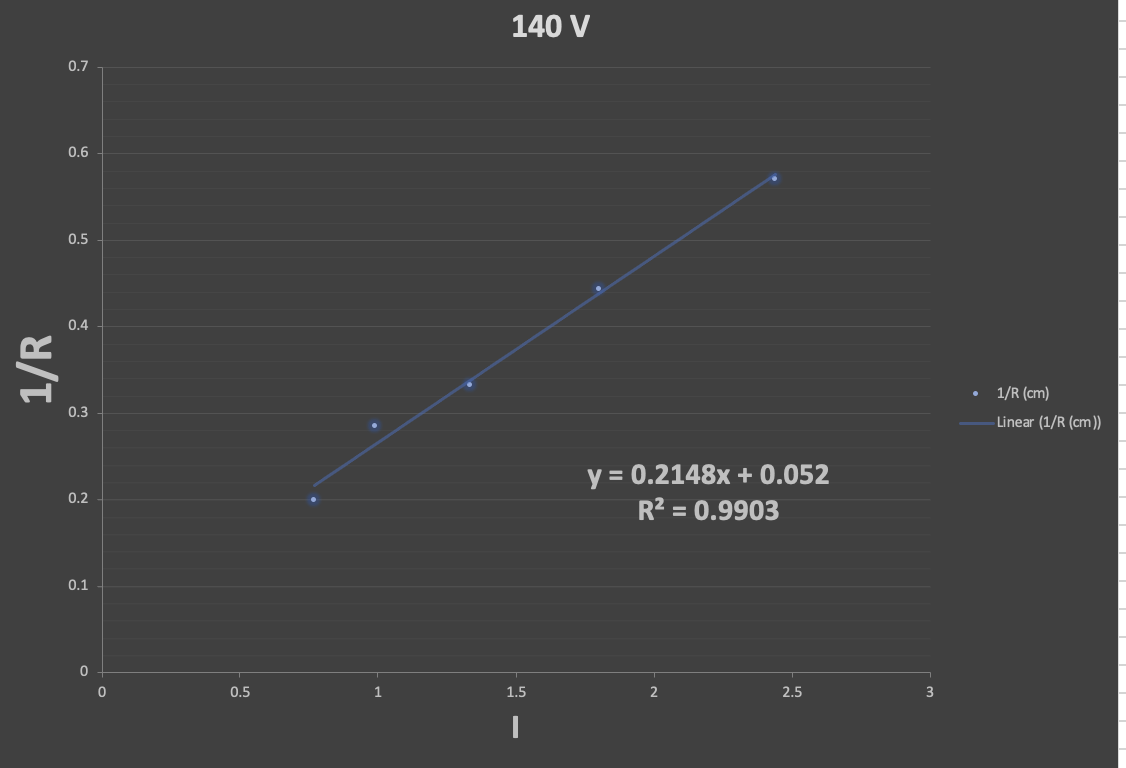
\includegraphics[scale=.7]{imagenes/3.png}
        \caption{140 V}
    \end{figure}
    \begin{figure}[H]
        \centering
        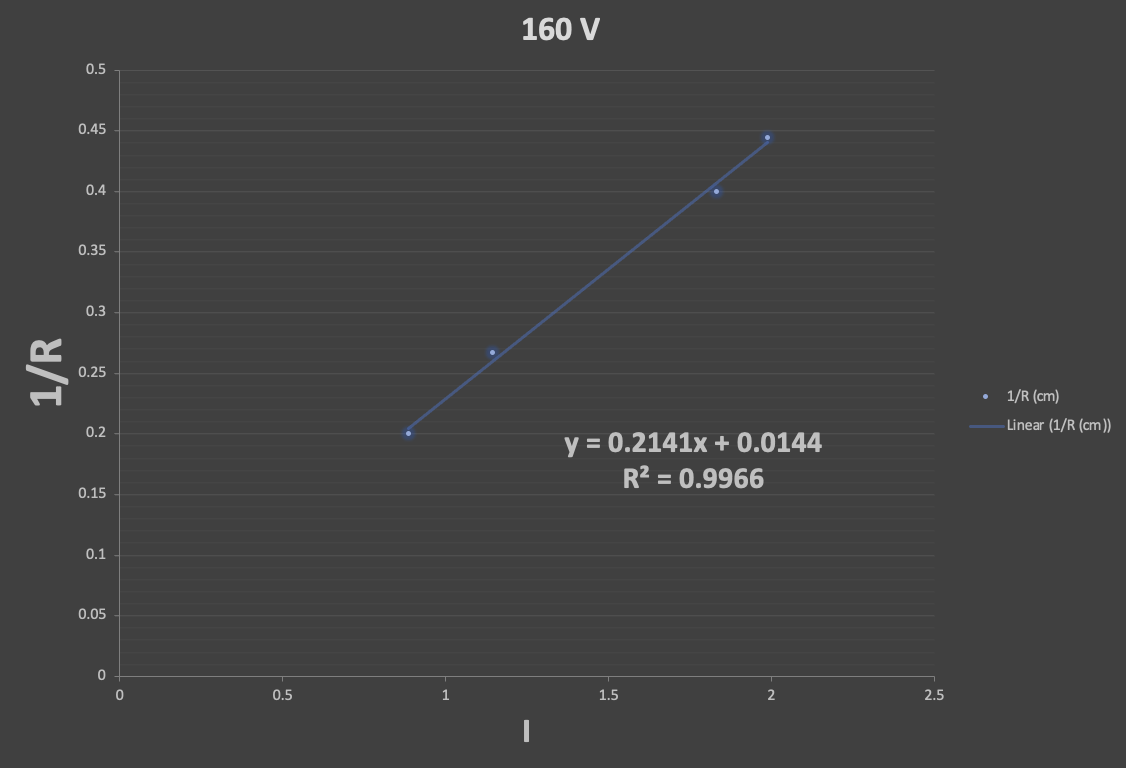
\includegraphics[scale=.7]{imagenes/4.png}
        \caption{160 V}
    \end{figure}
    \begin{figure}[H]
        \centering
        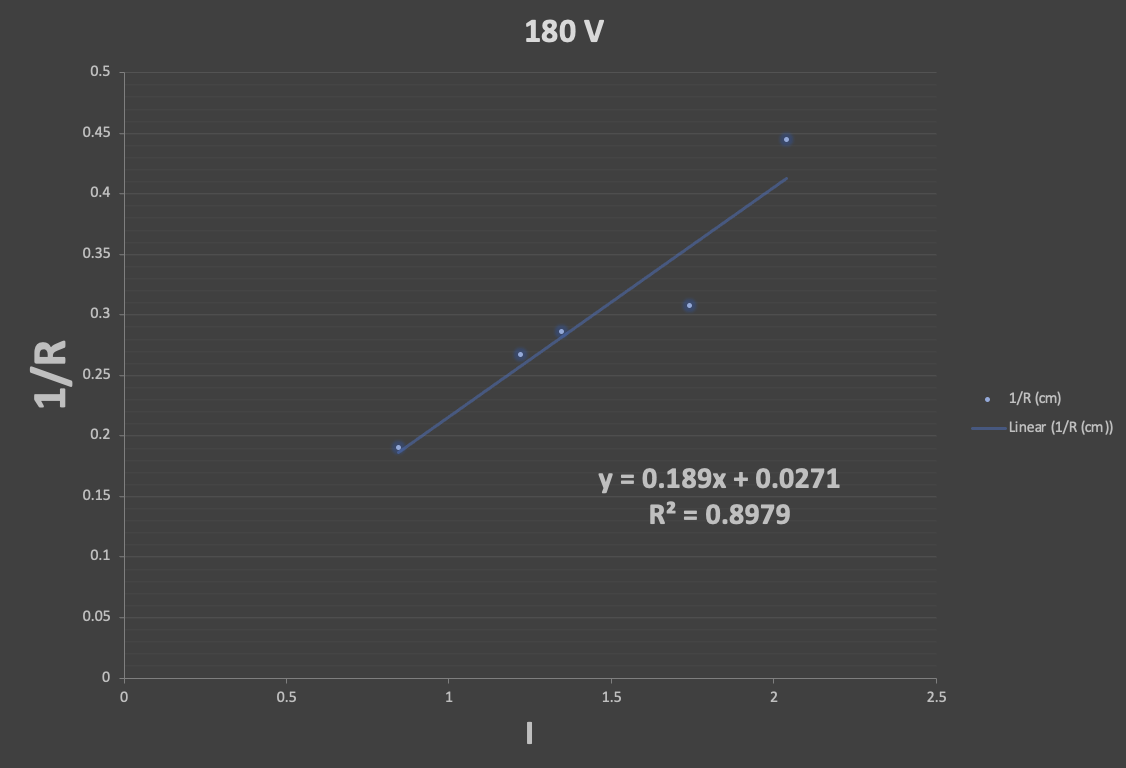
\includegraphics[scale=.7]{imagenes/5.png}
        \caption{180 V}
    \end{figure}
    \begin{figure}[H]
        \centering
        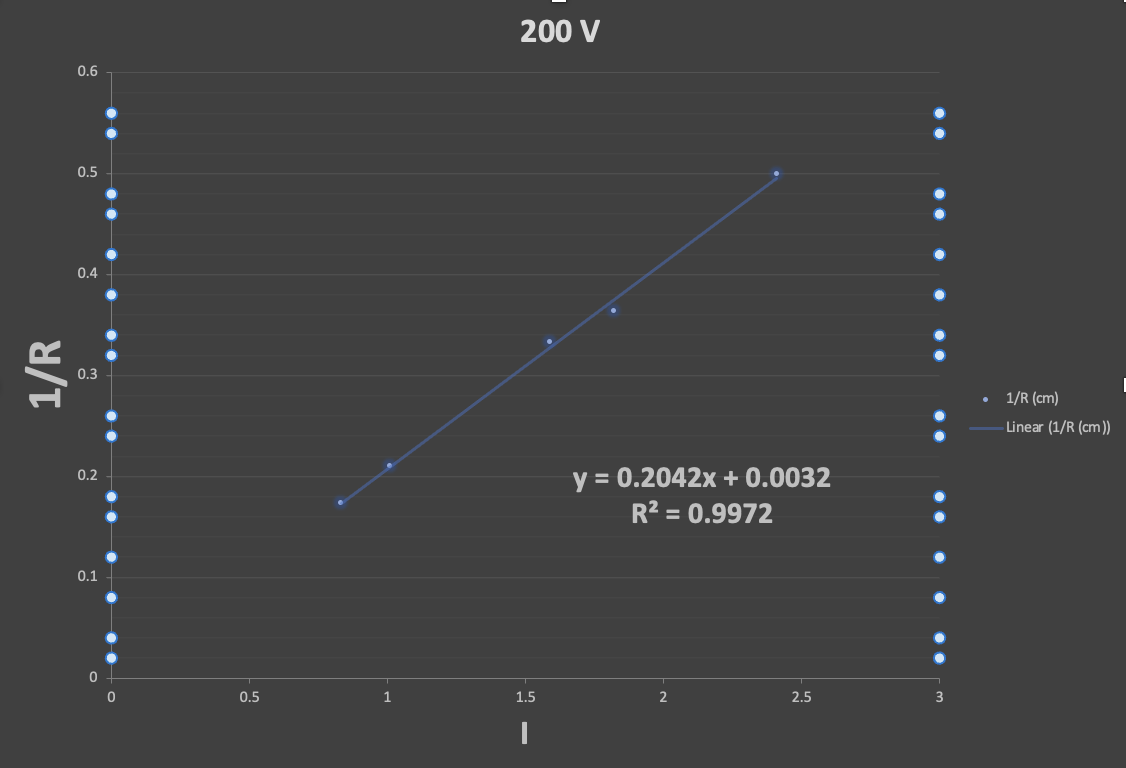
\includegraphics[scale=.7]{imagenes/6.png}
        \caption{200 V}
    \end{figure}

\section{Cálculo de $e/m_e$ para cada voltaje}

    Tenemos 
    $$\text{pendiente}=\frac{\mu_0 N }{a}\sqrt{\frac{32}{125 \Delta V}\cdot \frac{e}{m_e}}$$
    Despejando para $\frac{e}{m_e}:$
    $$\frac{e}{m_e} = \left(\frac{\text{pendiente}}{\frac{\mu_0 N }{a}\sqrt{\frac{32}{125 \Delta V}}}\right)^2 $$

    Con esta ecuación despejado la colocamos en Excel y obtenemos el $e/m_e$:

% Please add the following required packages to your document preamble:
% \usepackage{booktabs}
\begin{table}[H]
    \centering 
    \begin{tabular}{@{}ccc@{}}
    \toprule
    Voltaje & Pendiente & $e/m_e$     \\ \midrule
    100     & 0.2654    & 1266933.238 \\
    120     & 0.1835    & 504711.0163 \\
    140     & 0.2148    & 592778.4563 \\
    160     & 0.2141    & 515306.0543 \\
    180     & 0.189     & 356946.3919 \\
    200     & 0.2042    & 375001.8178 \\ \bottomrule
    \end{tabular}
    \end{table}

    \section{Porcentajes de error}

    % Please add the following required packages to your document preamble:
% \usepackage{booktabs}
\begin{table}[H]
    \centering 
    \begin{tabular}{@{}ccccc@{}}
    \textbf{Voltaje} & \textbf{Pendiente} & \textbf{$e/m_e$} & \textbf{Real} & \textbf{Porcentaje} \\
    100              & 0.2654             & 1266933.238      & 1.76E+11      & 99.9992795          \\
    120              & 0.1835             & 504711.0163      & 1.76E+11      & 99.999713           \\
    140              & 0.2148             & 592778.4563      & 1.76E+11      & 99.9996629          \\
    160              & 0.2141             & 515306.0543      & 1.76E+11      & 99.999707           \\
    180              & 0.189              & 356946.3919      & 1.76E+11      & 99.999797           \\
    200              & 0.2042             & 375001.8178      & 1.76E+11      & 99.9997867         
    \end{tabular}
    \end{table}

    De esto, se intuye que probablemente la ecuación sugerida en las instrucciones probablemente esté errónea, ya que los porcentajes de error son demasiado grandes. Pero considerando esto, el voltaje 100 fue el menor y el voltaje 200 fue el mayor. 

    %---------------------------

%\bibliographystyle{apa}
%\bibliography{referencias.bib}

\end{document}